\subsection{Схема Жиро}\label{section-girault-scheme}\index{схема!Жиро|(}
\selectlanguage{russian}

В схеме Жиро (\langfr{Marc Girault},~\cite{Girault:1990, Girault:1991}) надёжность строится на стойкости криптосистемы RSA (сложности факторизации больших чисел и вычисления дискретного корня).

Предварительно:
\begin{itemize}
    \item Доверенный центр (Трент, $T$):
    \begin{itemize}
        \item выбирает общий модуль $n = p \times q$, где $p$ и $q$ -- большие простые числа;
        \item выбирает пару из закрытого и открытого ключей $K_{T, \text{public}}: (e, n)$ и $K_{T, \text{private}}: (d, n)$;
        \item выбирает элемент $g$ поля $\mathbb{Z}_n^{\times}$ максимального порядка;
        \item публикует в общедоступном месте параметры схемы $n$, $e$ и $g$.
    \end{itemize}
    \item Каждый из легальных участников:
    \begin{itemize}
        \item выбирает себе закрытый ключ $s_i$ и идентификатор $I_i$;
        \item вычисляет и отправляет доверенному центру $v_i = g^{-s_i} \bmod n$;
        \item используя протокол аутентификации сторон (см. ниже) легальный участник доказывает доверенному центру, что владеет закрытым ключом, не раскрывая его значение;
        \item получает от доверенного центр свой открытый ключ:
            \[ P_i = (v_i - I_i)^d = (g^{-s_i} - I_i)^d \mod n; \]
    \end{itemize}
    В результате для каждого участника, например, Алисы, которая владеет $P_A, I_A, s_a$ будет выполняться утверждение:
        \[ P_A^e + I_A = g^{-s_A} \mod n. \]
\end{itemize}

Протокол аутентификации сторон в общем случае выглядит следующим образом (рис.~\ref{fig:key_distribution-girault-auth}).

\begin{figure}
    \centering
    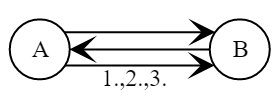
\includegraphics[width=0.5\textwidth]{pic/key_distribution-girault-auth}
    \caption{Взаимодействия участников в протоколе идентификации Жиро\label{fig:key_distribution-girault-auth}}
\end{figure}

\begin{protocol}
    \item[(1)] Алиса выбирает случайное $R_A$.
    \item[{}] $Alice \to \left\{ I_A, P_A, t = g^{R_A} \right\} \to Bob$
    \item[(2)] Боб выбирает случайное $R_B$.
    \item[{}] $Bob \to \left\{ R_B \right\} \to Alice$
    \item[(3)] $Alice \to \left\{ y = R_A + s_A \times R_B \right\} \to Bob$
    \item[(4)] Боб вычисляет $v_A = P_A^e + I_A$;
    \item[{}] Боб проверяет, что $g^ y v_A^{R_B} = t$.
\end{protocol}

Протокол генерации сессионного ключа, либо просто \emph{схема Жиро}, как и другие схемы, состоит из проходов обмена открытой информацией и вычисления ключа (рис.~\ref{fig:key_distribution-girault-scheme}).

\begin{figure}
    \centering
    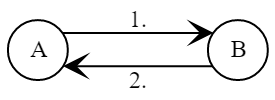
\includegraphics[width=0.5\textwidth]{pic/key_distribution-girault-scheme}
    \caption{Взаимодействие участников в схеме Жиро\label{fig:key_distribution-girault-scheme}}
\end{figure}

\begin{protocol}
    \item[(1)] $Alice \to \left\{ P_A, I_A \right\} \to Bob$
    \item[(2)] Боб вычисляет $K_{BA} = (P_A^e + I_A)^{s_B} \bmod n$.
    \item[{}] $Bob \to \left\{ P_B, I_B \right\} \to Alice$
    \item[(3)] Алиса вычисляет $K_{AB} = (P_B^e + I_B)^{s_A} \bmod n$.
\end{protocol}

В результате работы схемы стороны сгенерировали одинаковый общий сеансовый ключ.
\[ K_{AB} = (P_A^e + I_A)^{s_B} = (g^{-s_A})^{s_B} = g^{-s_As_B} \mod n; \]
\[ K_{BA} = (P_B^e + I_B)^{s_A} = (g^{-s_B})^{s_A} = g^{-s_As_B} \mod n; \]
            \[ K = K_{AB} = K_{BA} = g^{-s_As_B} \mod n. \]

Схема обеспечивает аутентификацию ключа (цель G7), так как только легальные пользователи смогут вычислить корректное значение общего сессионного ключа.

\index{схема!Жиро|)}